\PassOptionsToPackage{unicode=true}{hyperref} % options for packages loaded elsewhere
\PassOptionsToPackage{hyphens}{url}
%
\documentclass[]{article}

\usepackage{multirow}
\usepackage{graphicx}
\usepackage[]{algorithm2e}
% \usepackage{multirow}
 
 \usepackage[round]{natbib}
\usepackage{lmodern}

\usepackage{amssymb,amsmath}
\usepackage{ifxetex,ifluatex}
\usepackage{fixltx2e} % provides \textsubscript
\ifnum 0\ifxetex 1\fi\ifluatex 1\fi=0 % if pdftex
  \usepackage[T1]{fontenc}
  \usepackage[utf8]{inputenc}
  \usepackage{textcomp} % provides euro and other symbols
\else % if luatex or xelatex
  \usepackage{unicode-math}
  
  \usepackage{hyperref}
  \usepackage{cleveref}
  \defaultfontfeatures{Ligatures=TeX,Scale=MatchLowercase}
\fi
% use upquote if available, for straight quotes in verbatim environments
\IfFileExists{upquote.sty}{\usepackage{upquote}}{}
% use microtype if available
\IfFileExists{microtype.sty}{%
\usepackage[]{microtype}
\UseMicrotypeSet[protrusion]{basicmath} % disable protrusion for tt fonts
}{}
\IfFileExists{parskip.sty}{%
\usepackage{parskip}
}{% else
\setlength{\parindent}{0pt}
\setlength{\parskip}{6pt plus 2pt minus 1pt}
}
\usepackage{hyperref}
\hypersetup{
            pdfborder={0 0 0},
            breaklinks=true}
\urlstyle{same}  % don't use monospace font for urls
\setlength{\emergencystretch}{3em}  % prevent overfull lines
\providecommand{\tightlist}{%
  \setlength{\itemsep}{0pt}\setlength{\parskip}{0pt}}
\setcounter{secnumdepth}{0}
% Redefines (sub)paragraphs to behave more like sections
\ifx\paragraph\undefined\else
\let\oldparagraph\paragraph
\renewcommand{\paragraph}[1]{\oldparagraph{#1}\mbox{}}
\fi
\ifx\subparagraph\undefined\else
\let\oldsubparagraph\subparagraph
\renewcommand{\subparagraph}[1]{\oldsubparagraph{#1}\mbox{}}
\fi
\usepackage{cleveref}
% set default figure placement to htbp
 
\def\fps@figure{htbp}
\makeatother


\author{Meng Lu }
%date{Feb 2021}
\title{An agent-based model for human activity simulation and the assessment of personal exposure to ambient air pollution}
\begin{document}
\maketitle
\begin{abstract}
 
 Long-term exposure assessment to spatiotemporally highly variable air pollutants requires accounting for human space-time activity behaviours. Current advancement in activity-based exposure assessment are either buffer-based, which is achieved through different level of spatial aggregation, or are agent-based, such as those integrating with transportation models. which are commonly parameterised using activity diaries. The advantage of using an agent-based approach in flexibly representing space-time activities is obvious. However, for the current agent-based models, there is a trade-off between the simulation accuracy and the ability of the model to scale to long-term, large population simulation, and separating between different population groups based on their socio-economical profiles. This trade-off is what the proposed agent-based model attempt to bridge. We develop an agent-based model specific for air pollution exposure assessment and explicitly account for uncertainty from activities through representing different activities and possible locations as random variables, which enable repeated random sampling. As the model does not rely on detailed GPS tracks or mobile diary surveys but any statistical mobility data, the model is applicable to different scales, as well as for large sub-population groups and long-term exposure assessment. The model consists of three independent components: an activity simulation component, an optional air pollution prediction component, and an exposure assessment component that aggregates air pollution over the simulated space-time path based on the simulated activity schedules and the local environment of the locations. We demonstrate our model with the Dutch national mobile microcensus and high-resolution annually-average hourly NO$_2$ predicted from national ground stations. 

% in future, choose ABM dependsing on spatiotemporal variability of AP
% large-scale ABM with density functions. 
\end{abstract}

 
\section{Introduction}

%Chronic exposure to NO$_2$ poses a threat to public health, evidence has shown the negative effects of the NO$_2$ exposure to the cardiovascular and respiratory systems \citep{luo2016acute}. Despite public health concerns urging the attenuation of the negative effect of NO$_2$, the exact relationship between NO$_2$ exposure and our health remains unsolved. 
Highly traffic-related air pollutants such as NO$_2$ show considerable spatiotemporal variations at street levels. However, to understand the long-term or chronic health effects of NO$_2$ over a relatively large population (e.g. population of a city), most of epidemiological studies took a "static approach", which approximate the exposure as temporally averaged ambient pollutant concentrations at a person’s front-door home location. The same applies to risk assessment, the quantification of global, national, and local burden of diseases \citep{achakulwisut2019global}. It has been shown in many studies that for a spatiotemporally highly variable air pollutant, personal exposures assessed neglecting space-time activities, i.e. using concentration values at the front-door addresses, can differ considerably from personal exposures assessed accounting for human space-time activities \citep{duan1997combination,lu2019activity,park2017individual,molter2012performance,zenk2011activity}. \citep{yoo2015geospatial,yoo2021impact} took a step further to understand the joint effects of spatiotemporal mapping and space-time activities on exposure assessment, using respectively simulated and measured activity data. 

As measured activity data is hardly both over a long-term (e.g. a year or more) and a large population (e.g. millions). Activity simulation (commonly known as the "modelling approach") is needed. In transportation studies, progress has been made in the development of models for simulating transportation patterns, for example, the ALBATROSS \citep{ALBATROSS} is a transportation oriented system that simulates activities for the entire population based on activity diary data and dynamic constrains on scheduling decisions. Another relatively well-known activity simulation model is MATSim\citep{w2016multi}, which focuses on large-scale, one-day individual activity simulation based on a activity schedule scoring algorithm and detailed road networks. These activity models contribute to the understanding of human activity patterns \citep{miller2003prototype}. Many of these models are open-source \citep{w2016multi} and highly customisable, which allows scenario studies. The activity models consider a comprehensive set of space-time activity characters such as different travel means, work, education, and leisure activities, traffics \citep{w2016multi}. They are commonly parameterised by diary surveys consisting of locations visited and origin-destination schedules and estimate a continuous-time mobility track for each individual basing on general rules of human mobility patterns and space-time accessibility \citep{nguyen2011steps,gonzalez2008understanding,yang2010using,yu2006spatio,alessandretti2017multi,miller1991modelling}. Each route simulated can be contingent on, for instance, distance, safety, city infrastructure, and land use \citep{law2014measuring}. For example, \cite{shekarrizfard2017regional} assigned the predictions of a travel demand model to a road network to predict a person's hourly trajectories. For each person, the model selects a path from all possible paths by comparing the assigned travel time and the survey travel time. 


Integrating activity simulation models with predicted air pollution appear to be a solution to account for human space-time activities in exposure assessment. This has been reflected in several exposure studies \citep{shekarrizfard2017regional,deffner2016personal,gulliver2005time,dons2011impact}. A pioneered work is \cite{beckx2009dynamic}, who proposed to use the ALBATROSS to simulate hourly activities and then combine with an air dispersion model to assess exposure. However, none of these studies address long-term, uncertainty-quantified exposure assessment and for sub-populations. Specifically, \textit{long-term simulation} means the model is capable of quantifying exposure variations over longer times. \textit{Uncertainty} needs to be quantified for each simulated activity, including time schedules, travel modes, and possible destination locations. Separating \textit{sub population} groups allows more accurate simulation of their activities, as people's activity patterns may be clustered by their socio-economical status such as education, age, and occupation status. In another mindset, the confounders in health impacts studies such as age, gender, and living habits relate to certain space-time behaviours, but we only want to remove the effects of these confounders in health studies but not in exposure assessment, and this requires exposure assessment of sub-populations.  
%, which lead to bias in exposure assessment and thus the health study.

These three current limitations call for activity simulation models that are explicitly designed designed for exposure assessment. The framework developed in \cite{lu2019activity} attempts to address the first and second limitations. However, it assumes no activity information is available and therefore does consider population subgroups in real-life cases. We greatly extend from \cite{lu2019activity} to a new model which derives distributions of activity variables, namely travel modes and maximum travel distances, from national micro-census data. The new model is able to simulate closer to real-life exposures and greatly reduces uncertainty. The model has the following features: 

\begin{enumerate}
    \item Allowing flexible inclusion of irregular (e.g. holiday) activity schedules for long-term exposure modeling. 
    
    %\item The model can conveniently assimilate any other activity-related data, using either statistical modeling or . 
    
    \item Estimating or empirically specifying probability distributions for each activity based on  mobility surveys using statistical modeling for different population groups. 
    
    \item Sampling from the specified or estimated distributions repeatedly for uncertainty quantification and more accurate estimation of exposures through ensembling. 
    
         
\end{enumerate}

With this novel space-time activity model as the core component, we develop an activity-based NO$_2$ exposure assessment model consists of additionally an exposure assessment module and a temporal air pollution mapping module. The exposure assessment module takes output of the activity model, namely activity schedules and spatial locations of the activities (e.g. work locations, trip routes), and hourly NO$_2$ maps from the temporal air pollution mapping module to assess NO$_2$ exposures from each home location (\cref{fig:expflow}).     

\begin{figure}
    \centering
    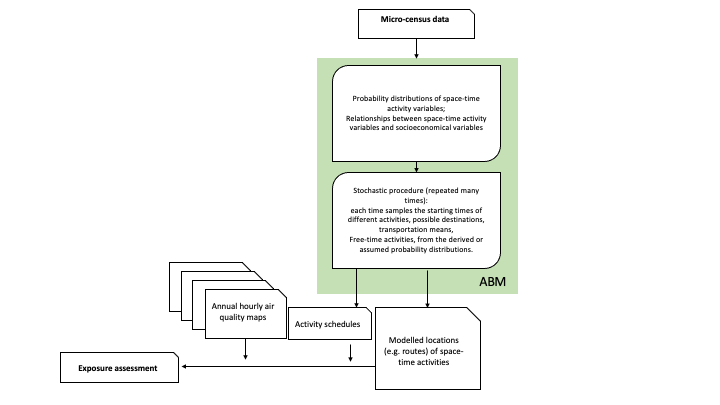
\includegraphics[width=\linewidth]{figure/exposureflow.png}
    \caption{The structure of our exposure assessment model. At the core is the agent-based human space-time activity model. ABM: agent-based modelling. }
    \label{fig:expflow}
\end{figure}



We follow the ODD (Overview, Design concepts, and Details) protocol \citep[][page 37,]{railsback2019agent} to describe our agent-based model. The OOD of our model is given in \cref{sec:model}, which follows with the exposure assessment model (statistical model in \cref{sec:exp}). Then, we demonstrate the modelling process for exposure assessment in a study case (\cref{sec:case}). The activity model is implemented with the Dutch national microcensus data and the exposure is assessed in the Dutch city of Utrecht, for the population group university student.  %\Cref{sec:result} shows the results in our study case. \Cref{sec:dis} discuss our models and the results. \Cref{sec:con} closes with a conclusion.


\section{Model overview and design concepts }
\label{sec:model}

\subsection{Overview} 

\textbf{Purpose}:
The model is developed for large population-scale (e.g. The entire population of the Netherlands), long-term, personal air quality exposure assessment accounting for human space-time activities. For this purpose, the model has three key features:
1) can simulating long-term behaviours with abnormal events (e.g. holidays),
2) explicitly assess uncertainty as human space-time activities commonly subject to high uncertainties.
3) can separate between population subgroups (e.g. with their age, sex, occupation status).

As the model is for large scale, we focus on deriving information from activity micro-survey data, in contrast to activity diaries and GPS tracks. These data may be employed for validation purposes. At a later stage, these data will be involved to dynamically improve the model.   

\textbf{Entities, state variables, and scales}:

The entities are each residence. The state variables include age, gender, occupation, income, working status (e.g. full-time worker or not), having children or not, having a car or not, and possibly other socioeconomical and environmental variables. The model is designed for long-term (one year or longer) exposure assessment over a population, focusing on a scale where land transportation (e.g. cars, bikes, on food) are the major commuting means. 

\textbf{Process overview}:

The most important task of the human space-time activity model (HSTAM) is to generate activity schedules (\cref{fig:detail}) for each home locations. The process is repeated several times (each repetition is called an iteration) for uncertainty quantification and improving the prediction accuracy of the exposure assessment.  In each interaction, the major steps are:   

\begin{enumerate}
    \item Specify the distribution of travel distances based on the survey data if the distribution is not pre-defined. 
    \item Sample from the distribution of the travel distances to choose a destination location from all possible destination locations.
    \item Based on the distance, it samples a travel mean according to the relationships identified between travel mean and travel distances, for different population groups  (e.g. old people, students) and travel purposes (e.g. going to work).
    \item A route is queried from OpenStreetMaps for the estimated travel mean. For example, a walk path is queried if the travel mean is by foot.  
    \item Based on the travel distances and travel mean, the duration is deducted. 
    \item Based on the duration, the end time of a trip or the start time of the next trip is estimated. 
    \item If the previous trip is not on a road, the start time of the trip is generated with a distribution. For example, the default departure time to work in our model is sampled from a Gaussian distribution with mean 8 (i.e. 8 am) and standard deviation 0.2. 
    \item The free time activities are randomly sampled from a set of activities, for example, staying at home or take a walk. 
\end{enumerate}

\Cref{fig:detail} illustrates how an activity schedule is generated. 

\begin{figure}
    \centering
    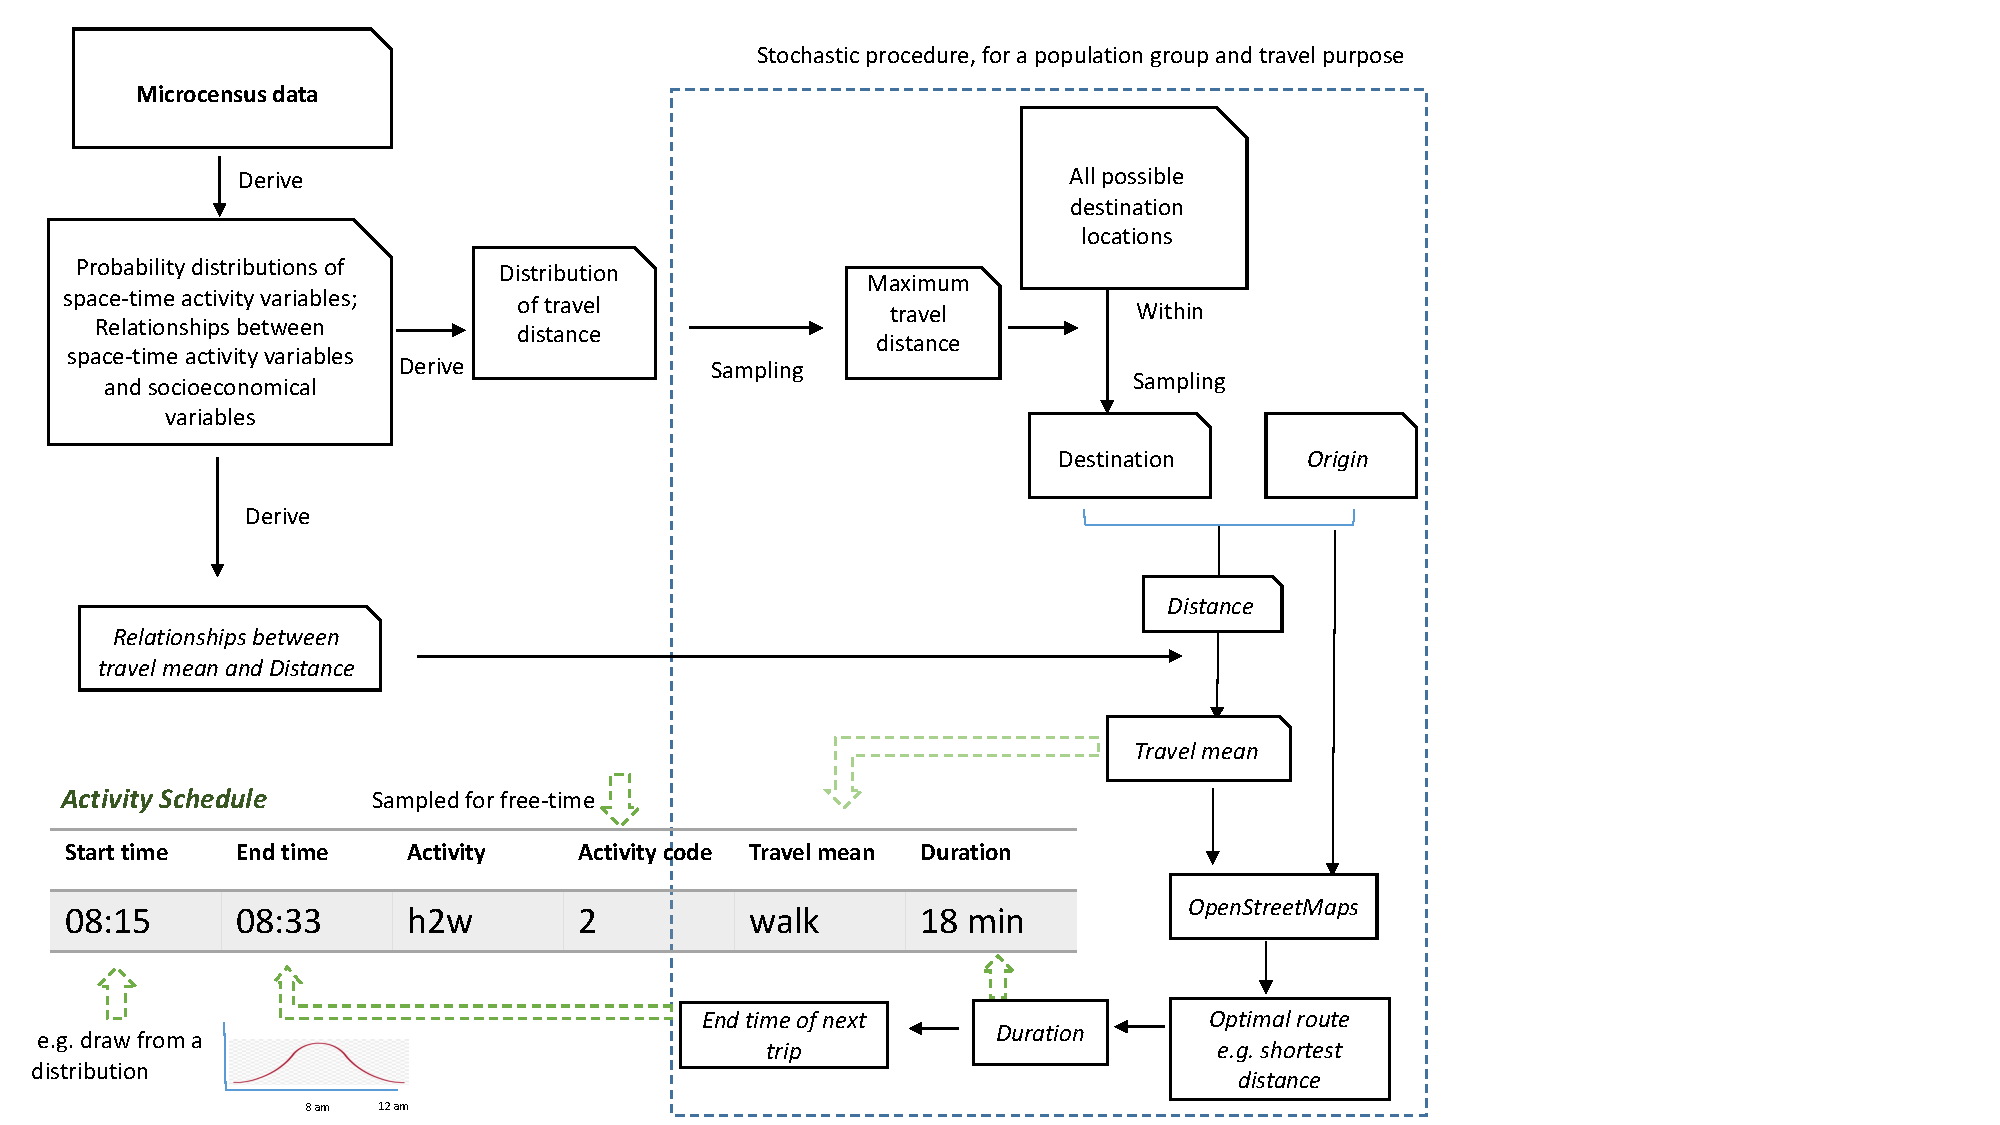
\includegraphics[width=\linewidth]{figure/scheduleflow_noenrich.pdf}
  \caption{Procedure of generating activity schedules using the human space-time activity model}
    \label{fig:detail}
\end{figure}

\subsection{Design concepts}
The basic concept of the proposed model is the travel behaviour simulation. The simulation is based on probability distributions of agents' travel mode, maximum travel range, classified by their socio-economic status. The distributions are derived from microcensus data. By the probabilistic nature, stochasticity is used. In each iteration, the departure time of an activity , travel mode, maximum travel distance, possible destination locations, and the free-time activities may all change. This allows uncertainty quantification as well as a more accurate estimation of long-term behaviour through averaging. 


\subsection{Model Details}
\subsubsection{Input and output of the model}

The input of the HSTAM consists of 1) home locations to estimate. 2) All the possible destination locations for each destination type (e.g. all the work locations, all the school locations). 3) A table indicating the probability each travel mean is taken for different distances and for different population groups and travel purposes. 4) The distributions of the travel distances for certain population groups, either pre-defined by the user, i.e., the distribution is the input, or predicted from survey data, i.e. the survey data is the input.
 

The HSTAM generates activity schedules and spatial locations and tracks of the activities, for each iteration and each individual. The activity schedule consists of, for each trip, a start time, an end time, the travel mean, the duration, as well as the activity name and a corresponding code. \Cref{tab:sche} shows an example. The spatial locations of the activities, as well as the properties of trips, including the speed, means, duration of a trip, the total number of locations a destination is drawing from, are stored in the OGC GeoPackage format. 

\begin{table}[]
\resizebox{\textwidth}{!}{%
\begin{tabular}{cccccc}
\\[-1.8ex]\hline 
\hline \\[-1.8ex] 
start\_time & end\_time & activity   & activity\_code & travel\_mean          & duration                   \\ \hline
0.0         & 7.06      & home       & 1              & \multirow{7}{*}{foot} & \multirow{7}{*}{335.55672} \\
7.07        & 7.17      & h2w        & 2              &                       &                            \\
7.18        & 16.14     & work       & 3              &                       &                            \\
16.15       & 16.23     & w2h        & 2              &                       &                            \\
16.24       & 17.73     & home       & 1              &                       &                            \\
17.74       & 19.73     & free\_time & 1              &                       &                            \\
19.74       & 23.9      & home       & 1              &                       &     \\ \hline                      
\end{tabular}%
}
\caption{An example of activity schedules. h2w means "home to work", and w2h means "work to home". The "bicycle" indicates the transportation mean, which is generated from the activity model. The integer part indicates hours, and the digits indicate minutes in percentage, e.g., 9.89 is at around 9:54 am (54 = 89*0.6).}
\label{tab:sche}
\end{table}
 
 


\subsubsection{A built-in dataset}
\label{sec:data} 
For demonstrating the parameterisation of each module of the model, and for guiding the application of the models, we include a dataset in the model. The dataset origins from the long-term Dutch national travel survey, OViN (2010 - 2017, followed by OVG and MON)). OViN is collected by Statistics Netherlands (in Dutch: Centraal Bureau voor de Statistiek - CBS) for one-day trip-based diary. It consists of 0.3 of the Dutch population. The preprocessing of the dataset includes parsing the text of variables (as shown in \cref{preprocess}) to extract the range of the data and calculate a mean of the data range. The variables, their original text, and generated variables are listed in \cref{preprocess}.
% Please add the following required packages to your document preamble:
 

\begin{table}[!h]
\resizebox{\textwidth}{!}{%
\begin{tabular}{l|l|l|l|l|l}
\hline
Variable       & original variable name & \begin{tabular}[c]{@{}l@{}}example of the \\ variable content\end{tabular}                           & new variables                                                                     & \begin{tabular}[c]{@{}l@{}}new \\ variable\\  value\end{tabular} & note                                                                                                                                                              \\ \hline
Trip distances & KAfstR                 & \begin{tabular}[c]{@{}l@{}}"5,0 tot 7,5 km"\\ "50 km of meer"\\ "Geen rit in Nederland"\end{tabular} & \begin{tabular}[c]{@{}l@{}}KAf\_low\\ KAf\_mean\\ KAf\_high\end{tabular} & \begin{tabular}[c]{@{}l@{}}5\\ 6.25\\ 7\end{tabular}             & \begin{tabular}[c]{@{}l@{}}"geen rit in\\  Nederland" \\ means the trip \\ is not in the \\ Netherlands \\ and is not \\ considered \\ in this study\end{tabular} \\ \hline
Income         &                        &                                                                                                      &                                                                                   &                                                                  &                                                                                                                                                                   \\ \hline
Age            &                        &                                                                                                      &                                                                                   &                                                                  &                                                                                                                                                                   \\ \hline
...            &                        &                                                                                                      &                                                                                   &                                                                  &                                                                                                                                                                   \\ \hline
\end{tabular}%
}
\label{preprocess}
\end{table}
 
\subsubsection{Probabilistic components}
The details of generating the components that are probabilistic are given below. %The model includes a built-in dataset of the Dutch national microcensus data called OViN. A description of the dataset is seen in \cref{sec:case}.

\begin{enumerate}
\def\labelenumi{\arabic{enumi}.}
\item
  Activities:
  \emph{Work-day activities:} 1) home, 2) home to work, 3) work, 4) work
  to home, 5) sports. The assumption for sports is that it occurs in the
  morning or evening, and it occurs either 1 hour before departure to
  work or 1 hour after come back home from work.

  \emph{Weekend activity}: 1) shopping, 2) random walk 
\item
  A \textbf{probailistic} model: the components below are probabilistic,
  and the distributions can come for activity surveys or literature.

  1) \underline{Time schedule:} please see section 2 for the activities.
  The departure times to work and back from home are probabilisitic. By
  default, a gaussian distribution is used (e..g with mean 8 and
  standard deviation 0.5 for going to work). In our implementation, the
  distributions of departure times are fitted (characterised) from human
  activity surveys (please see section 4 below). The distributions are
  fitted for each population group.

  2) \underline{Unknown destination locations:} For large-population
  activity modeling, it is commonly the case that the specific
  destination location (e.g. work location, sport centres) are unknown
  for each individual. However, the information for the entire locations
  (e.g. sport centres, work buildings, universities, schools) are
  becoming more comprehensive. In many countries, this part of
  information can be acquired from OpenStreetMaps. In this study, we
  select potential locations by proabilisticly sampling the maximum trip
  distance and only randomly select locations within the Euclidean
  distance of the maximum trip distance. If there is no destination
  points within the sampled maximum trip distance, the nearest
  destination point is used. The number of total selected destination
  points serve as an uncertainty indicator in the situation of unknown
  destination locations, in each simulation run.

  3) \emph{\underline{Means of commuting}} (currently: (train),
  autovehicles (car, bus, tram), bike, on foot): are deteremined based
  on travel distance. Based on the population group (e.g. school
  student) and the travel purpose (to school), the probability that a
  certain travel mean is taken is calculated (e.g. 0.3 for on foot and
  0.6 for biking, 0.1 for taking a bus or car and 0 for others),
  according to which a travel mode is sampled in each simulation. The
  commuting routes are queried from OpenStreetMaps.
\item


  Implementation:

  Population group implemented are: school student (U17) , University
  student (students older than 18 years old, Uni), part-time worker
  (PW), full-time worker (FW).

  There is a conceptural default implemented in our model which is
  described in table 1. In our case-study (Utrecht) implementation, they
  are characterised from Dutch national activity surveys (OVin). The
  process is: 1) we select a profile (e.g. Univeristy student) and a
  purpose (e.g. go to work), 2) we fit the distribution of the selected
  data. 3) At each simulation, we sample one value from the
  distribution. Specifications are described below:

  \textbf{Destination location selection:}
\end{enumerate}


\begin{itemize}
\item
  Default: randomly pick a location.
\item
  OVin: probability counted from means of \emph{commuting vs. distance}.
  for each population group (but not specified with travel purpose).
\item
  Profile implemented: School students (U17), University students (Uni),
  PW, FW; for going to work (including all functional non-residential
  buildings, data same as the Utrecht paper), going to universities
  ((locations from OSM), going to schools (locations from OSM).

  \textbf{Means of commuting}:
\item
  Default: conceptural probabilistic model for going to work.
\item
  OVin: probability counted from means of \emph{commuting vs. distance}.
  for each population group (but not specified with travel purpose).
\item
  Profile implemented: School students (U17), University students (Uni),
  PW, FW.

  \textbf{Departure time to work:} 
\item
  Default: gaussian model with mean 8 and standard deviation (SD) 0.5.
\item
  OVin: Distribution characterised: departure time (KVtijd). 
\item
  Profile implemented \emph{(Todo)}: School students (U17), University
  students (Uni), PW, FW. 
\end{itemize}


\section{Study case: activity modeling using the Dutch national microcensus data}
\label{sec:case}
The example below shows how we model the profile group: school student (U17). The activities considered are 1) going to school, 2) staying at school, 3) going back home, 4) going to a sport center, 5) going back home.  


%Firstly, we characterise the distribution of the distances between home location and a work location. 
\textbf{Selecting the locations of school and sport centres.}

We demonstrate here the selection of the school location for each individual considered, selecting the location of a sport centre follows the same procedure.   
\begin{itemize}
    \item Step 1: histogram analysis and model fitting. \\ From the histogram of the travel distances between student's home location and work (i.e. school) location \cref{stu_work_hist}, we can observe that the original distribution is log-normal or power law. The log transformed distribution is visually close to a normal distribution. We therefore fit both models and at last decided on a log-normal. We conducted a Shapiro test to prove the log-normal distribution.  
    
    \item Step 2: distance sampling. \\ In each simulation step, we randomly sample a distance from the fitted log-normal distribution.
    
    \item Step 3: Select candidate/potential destinations. \\ The sampled distance is regarded as the maximum travel distance (MTD), all the possible locations (i.e. all the schools) within the Euclidean distance of the MDT are considered as the "candidate destinations". (As the actual routes have a longer distance, this can be seen as an a bit conservative way of selecting potential destinations). 
    
    \item Step 4: Randomly sample one location from all the potential destinations.
    
\end{itemize}
\begin{figure}[!h]
    \centering
    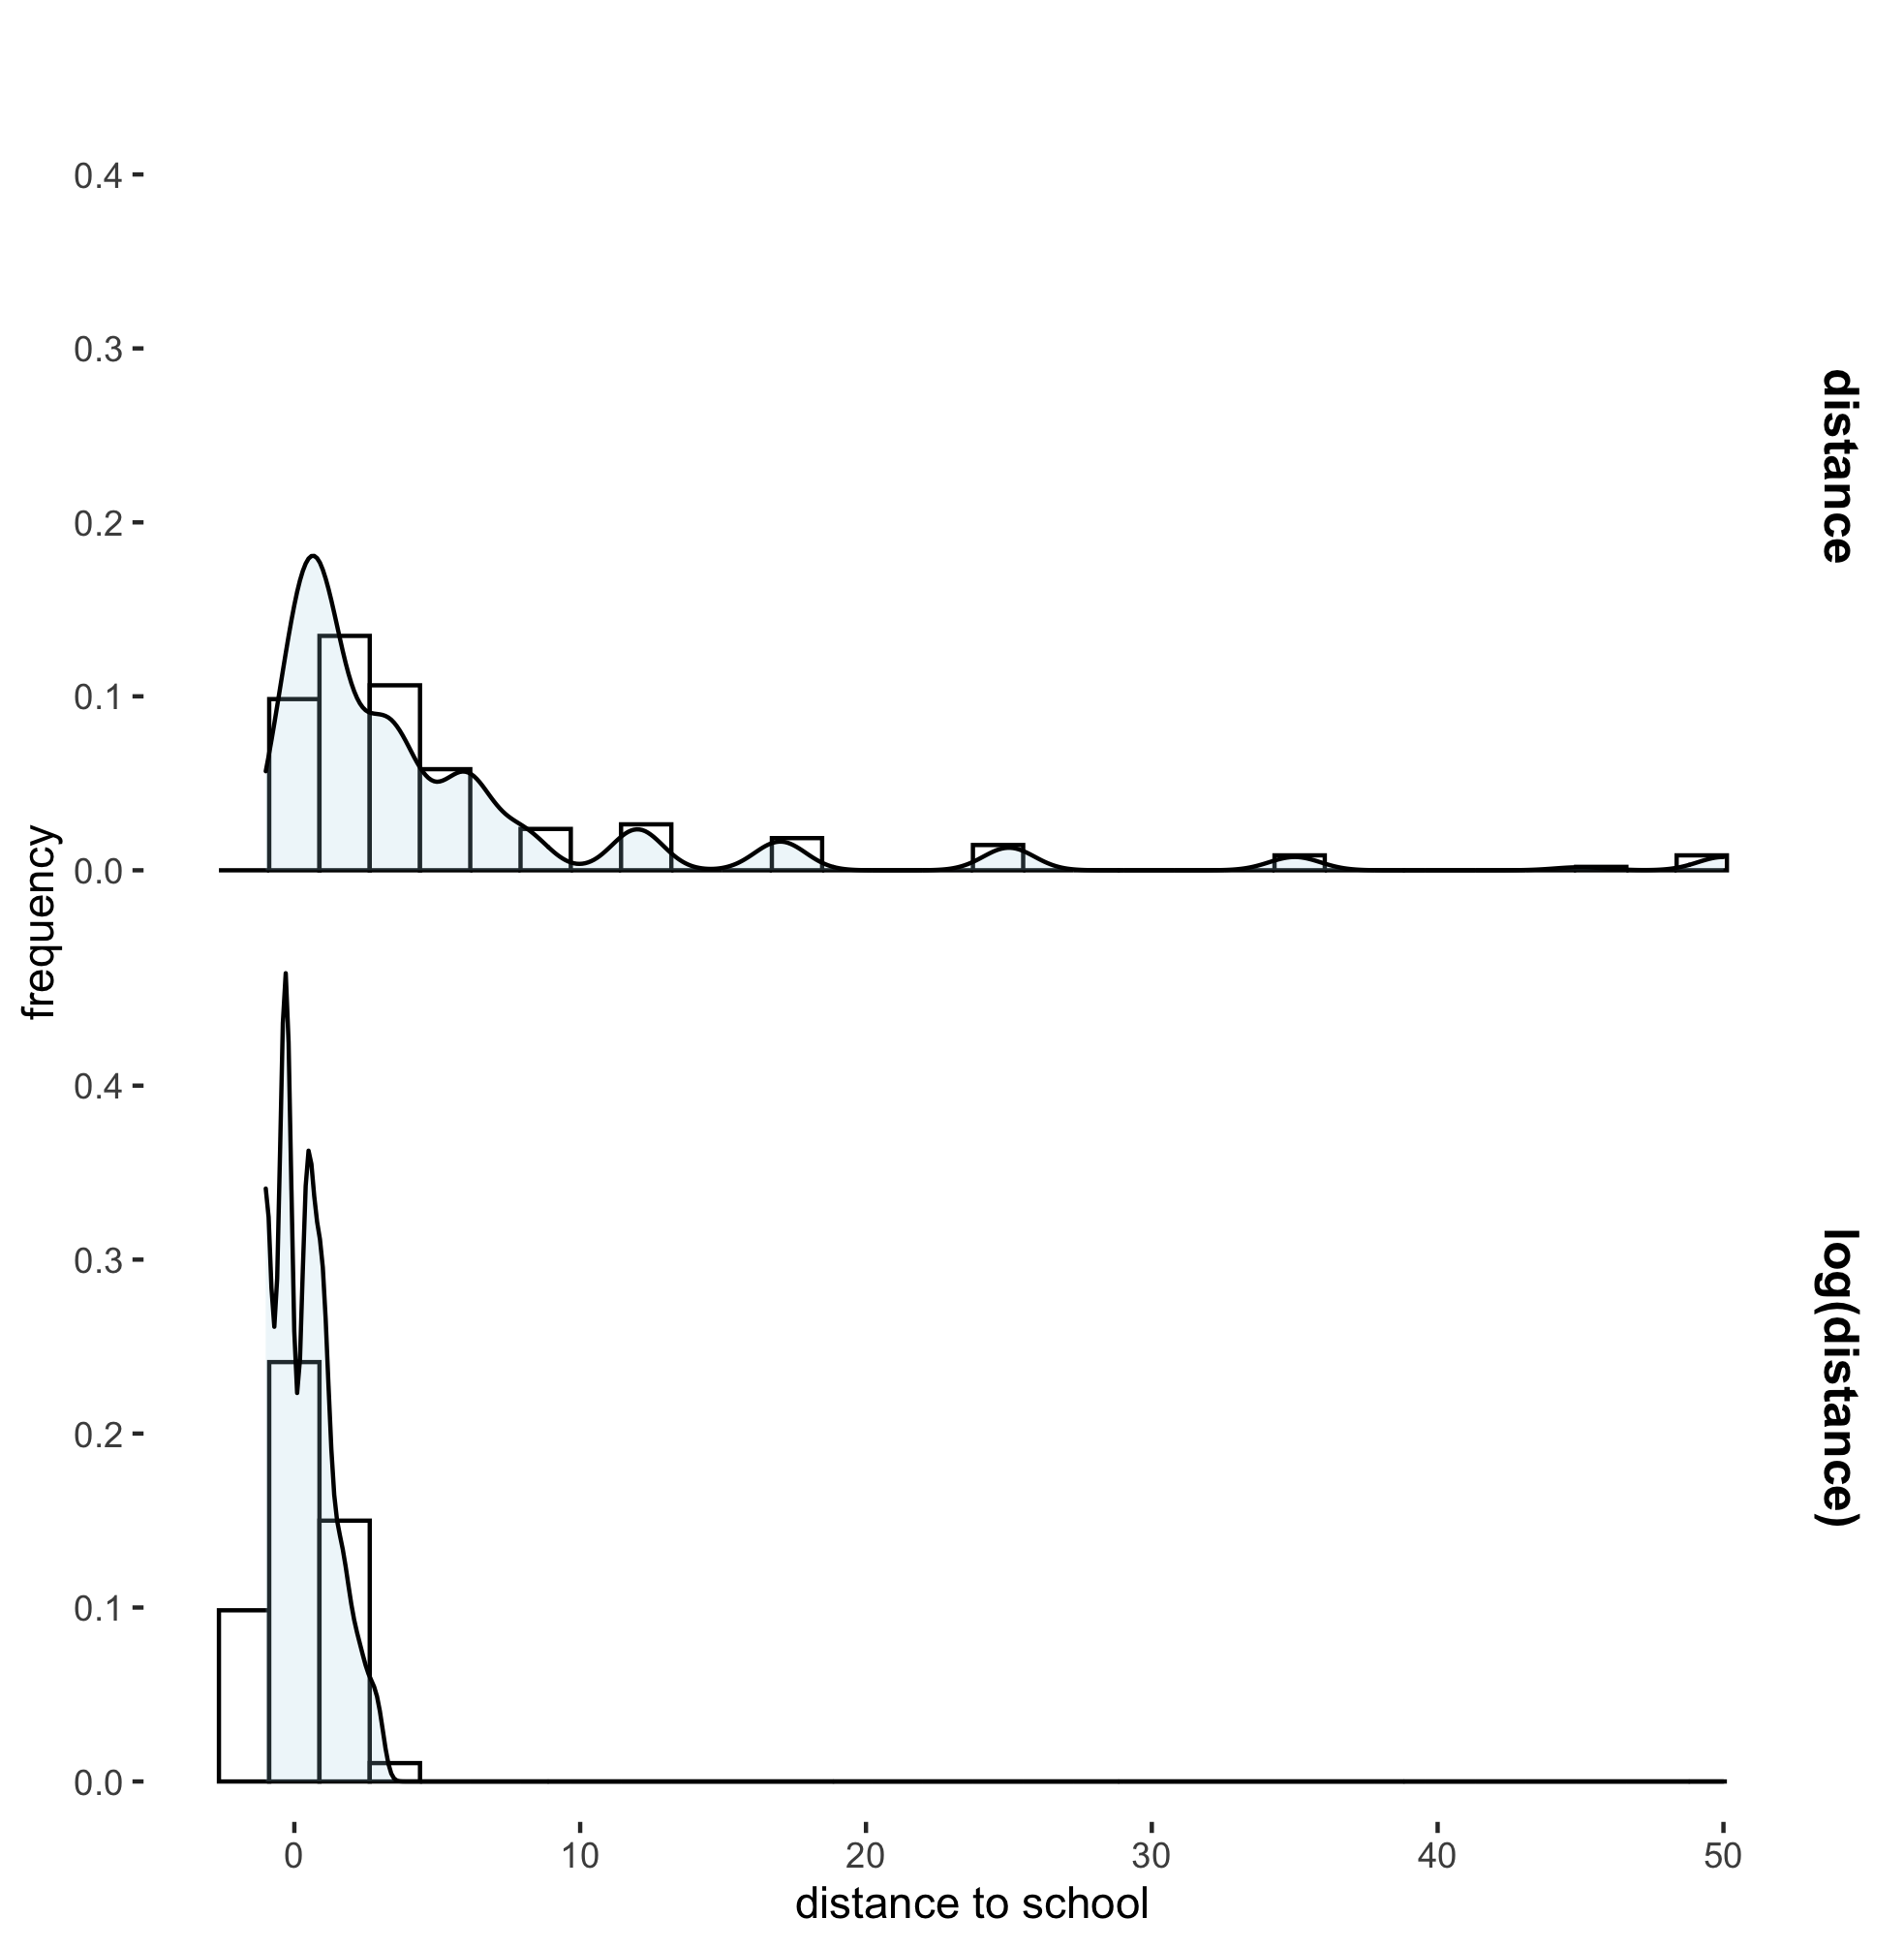
\includegraphics[width=8cm]{figure/ditance_to_school.png}
    \caption{Histograms and density plots of the distances between students' home location to work locations. }
    \label{stu_work_hist}
\end{figure}

\begin{figure}[!h]
    \centering
    \includegraphics[width=8cm]{figure/buffer.png}
    \caption{Example of selecting a sport location. The triangles indicates all the sport facilities. Only the locations within the maximum travel distances are considered, i.e. the green triangles within the buffer. And from them, one of the location is randomly sampled, marked as the \textit{Ping-pong racket and ball}. }
    \label{buffer}
\end{figure} 

An alternative way to replace step 3 and 4 is to calculate the distances between the original location and all the destination locations, and directly sample a location. This method is computationally much more intensive. 

\textbf{Choosing the transportation mean}

Now we have the home location and the destination (i.e. sport centre, school) locations, the second step is to choose the transportation mean based on the trip distance. 

\begin{itemize}
    \item Step 1: regroup transportation means and the travel distance range. \\ We regrouped the transportation means to bike, train, walk, and auto vehicles, which include all the other transportation vehicles (bus, tram, car,...). We regrouped the travel distance range as shown in \cref{stu_mode_dist}. 
    
    \item Step 2: calculate the probabilities of the transportation means within each travel distance range. \\ we count for each travel distance range the incidence of each transportation mean, and divided by the total incidence of each travel distance range to obtain the probability (of the transportation mean in each travel distance range).
    
    \item Step 3: sample the transportation mean. At last, based on the travel distance, which is calculated from the OpenStreetMap walking routes \footnote{we use the walking routes as this is commonly shorter than other routes, if this is already long, then the person has a very high probability of taking a car} based on the original location (e.g., home) and the destination (e.g., school), we sample a transportation mean given the probability.   
    
\end{itemize}

\begin{figure}[h]
    \centering
    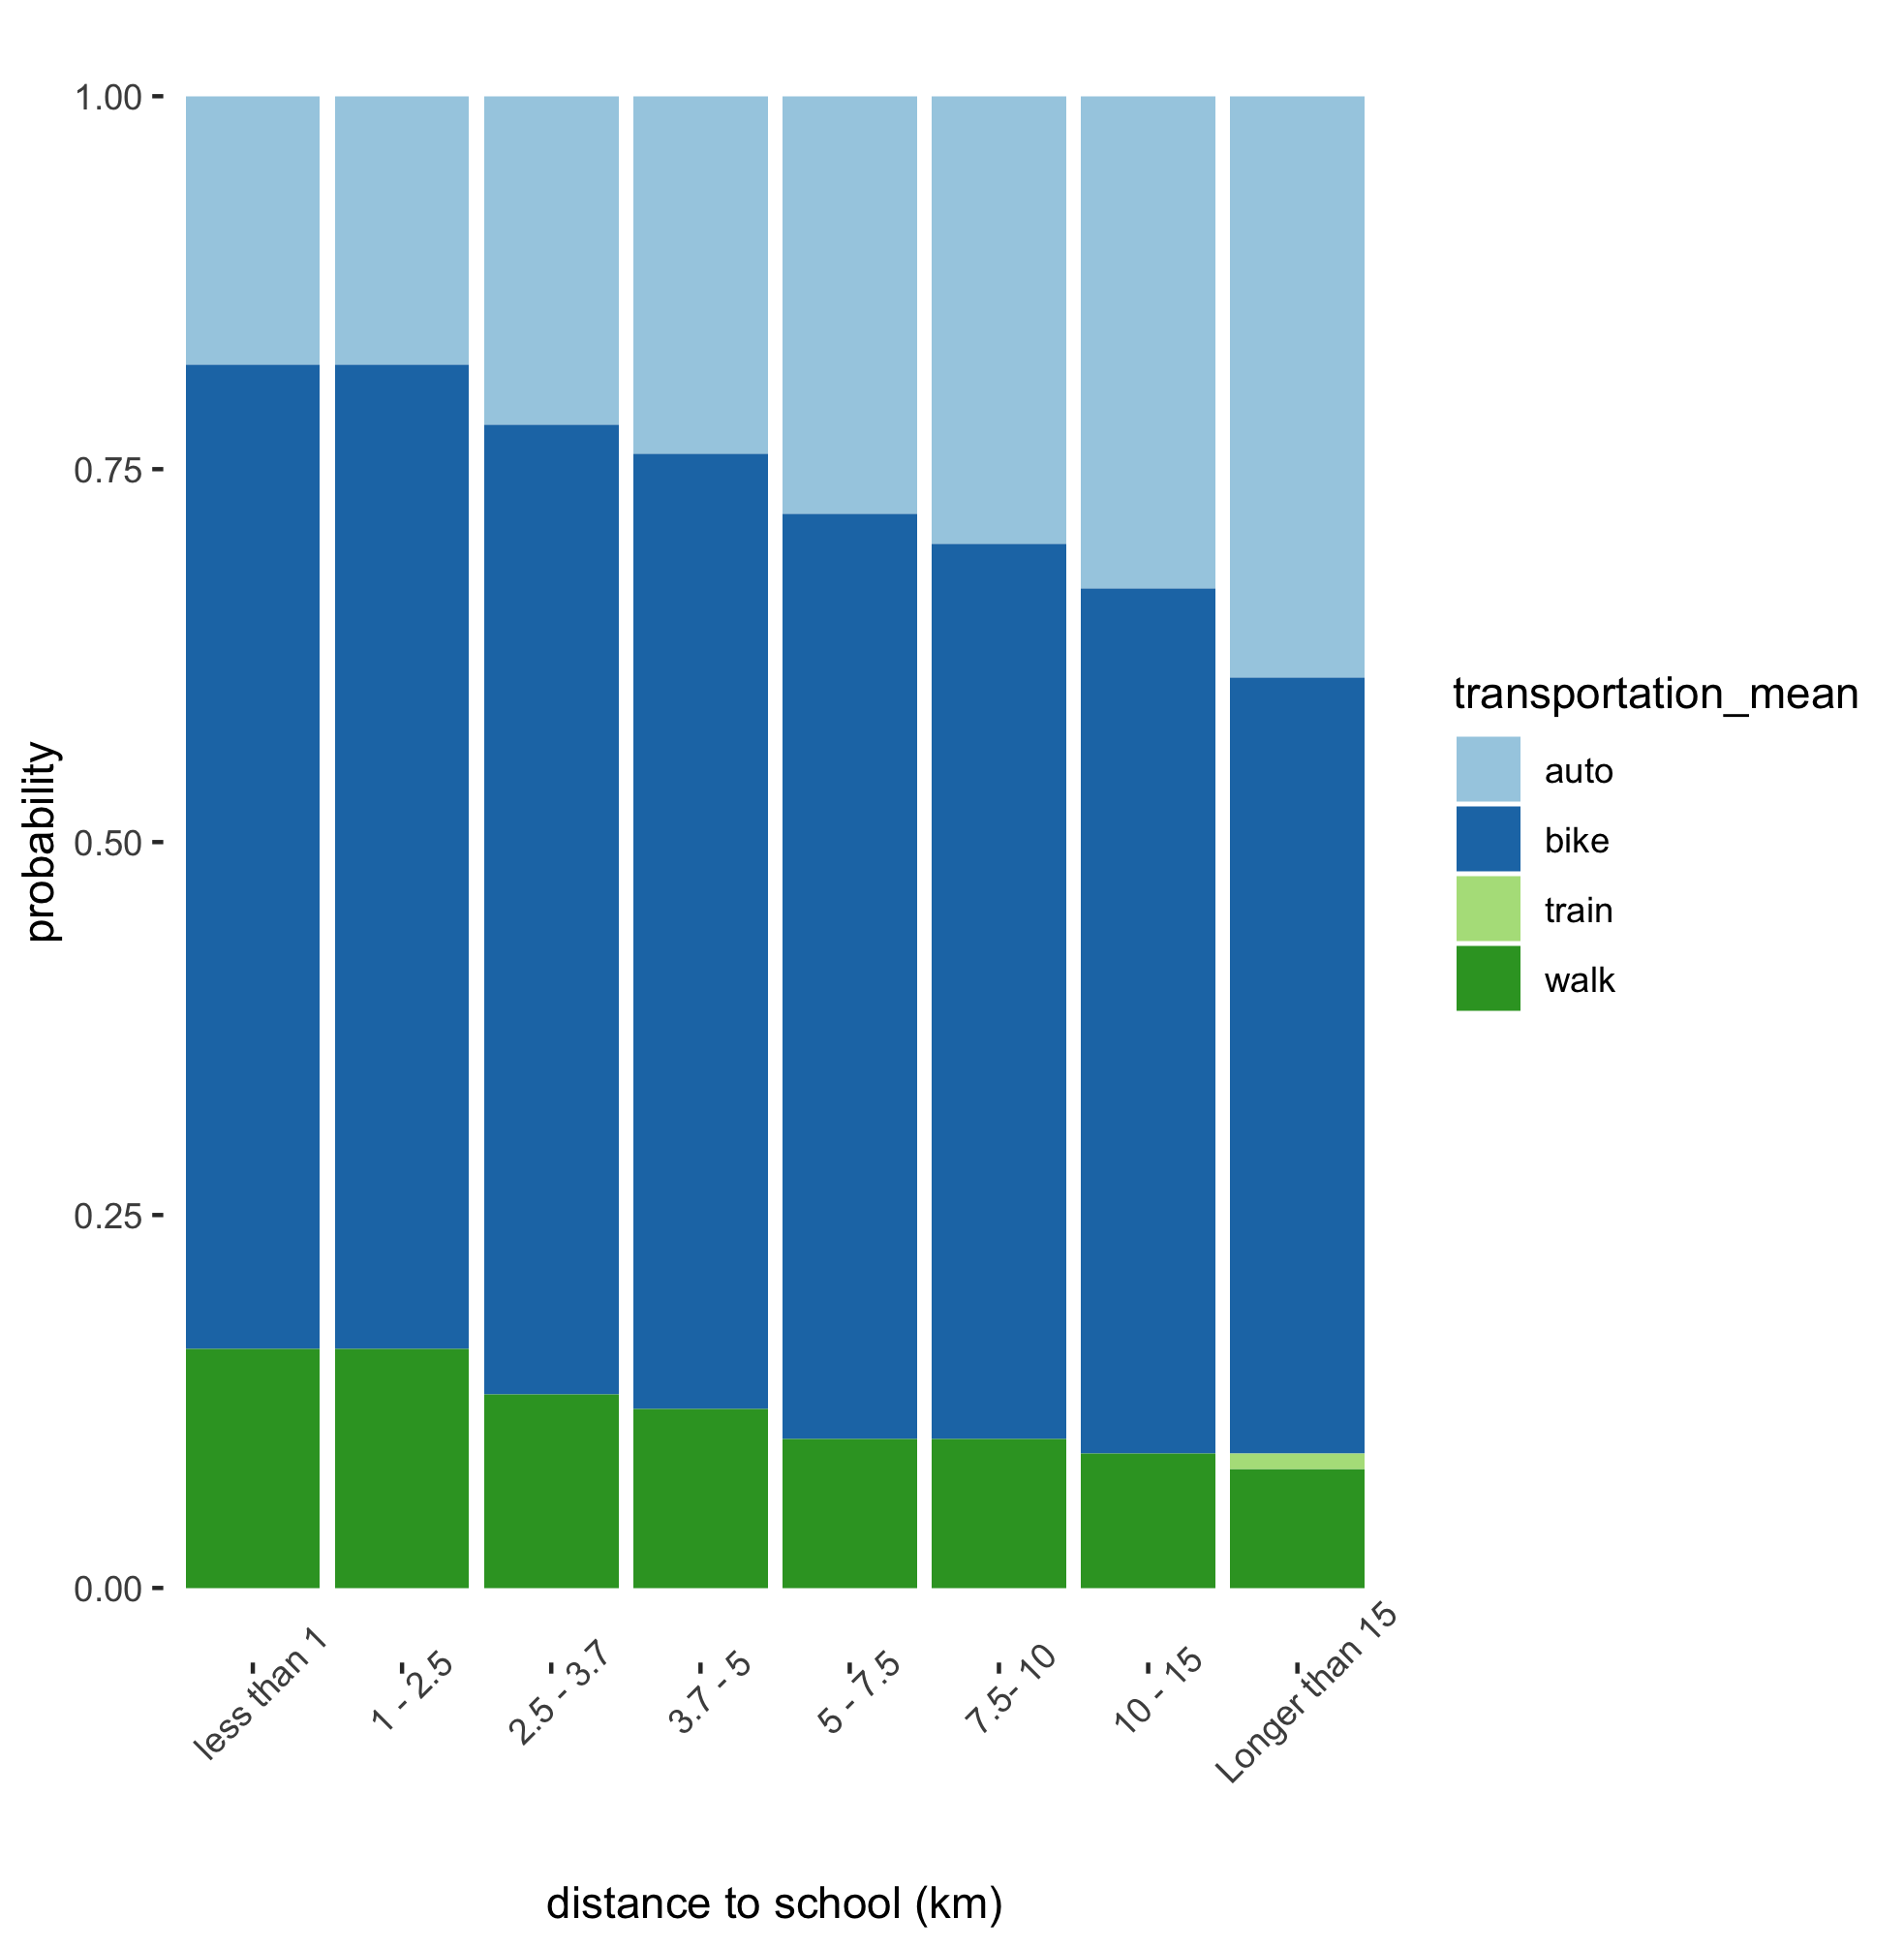
\includegraphics[width=8cm]{figure/ditance_vs_transmean_schoolstud.png}
    \caption{Probability of the transportation mean with regard to trip distance ranges for students (U17). The trip distance ranges are re-scaled from the original travel distance. The transportation means are re-grouped from the transportation means in the Ovin survey.}
    \label{stu_mode_dist}
\end{figure} 

\textbf{Generating the activity schedule and geospatial information (e.g. routes)}

Based on the transportation mean, we query the OSM route and the travel time accordingly. E.g. if the transportation mean is "bike", then we use the bike routes. With the travel time to each destination, we can complete our schedule with the starting time and the ending time of each activity. There are two ways of generating the time of going to school, as described in the section \textit{Time Schedule} above. An example simulated schedules look like \cref{schedule,schedule2}. An additional "Geometry" will be added to link the activity with the geographical points (e.g. front door location), lines (e.g. routes), or polygons (e.g. buffers). An example is shown in \cref{exampleroute}.
\begin{figure}[!h]
    \centering
    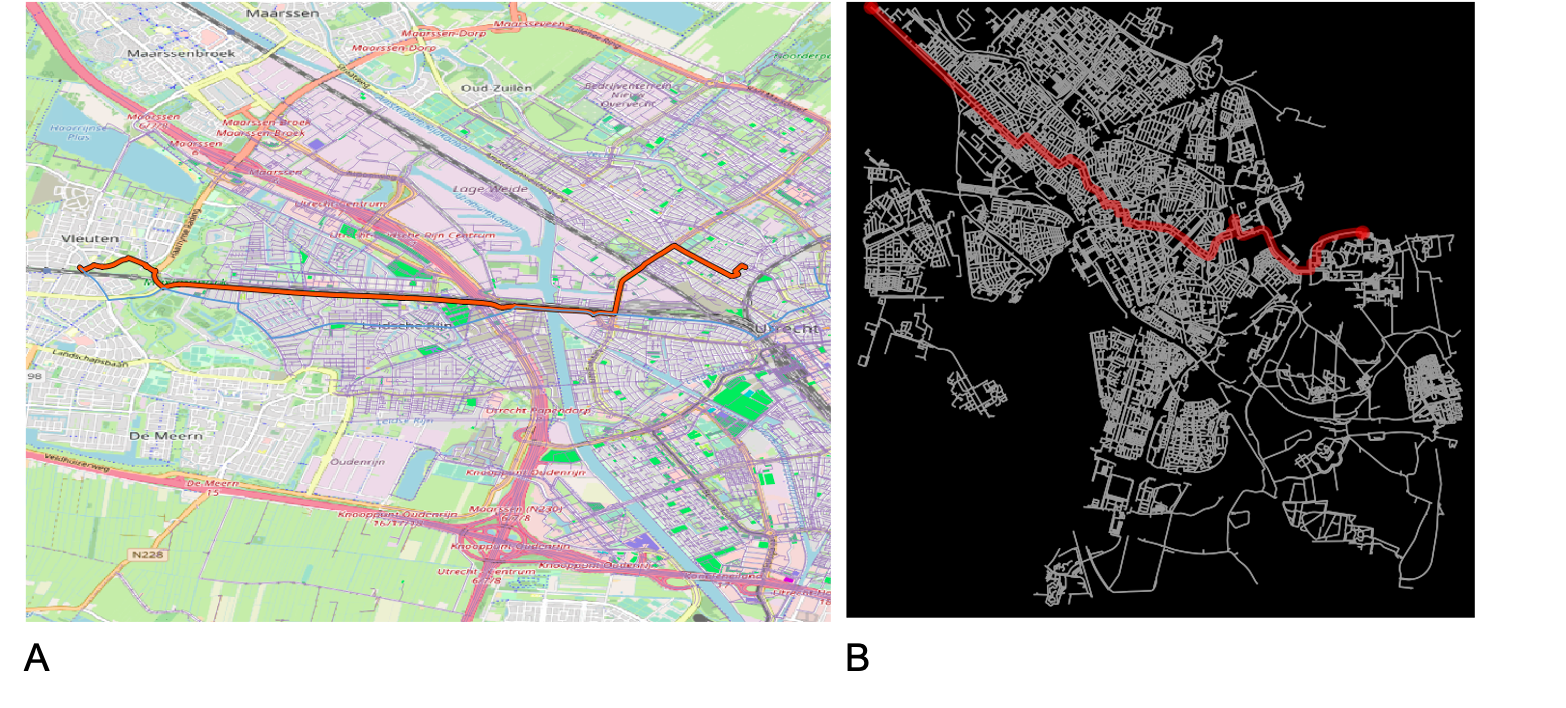
\includegraphics[width=10cm]{figure/route.png}
    \caption{Example of routes queried from the OpenStreetMaps of an individual taken from home to work, in the city of Utrecht. A route with the shortest travel time is selected for travelling on drive ways, and a route with shortest travel distance is selected for on bike and walk ways. A: bike route, B: drove route.}
    \label{exampleroute}
\end{figure}
%


\section{Exposure assessment model}
\label{sec:exp}
 Based on the activity model, we develop an Exposure assessment model, which consists of three components:
 \begin{enumerate}
     \item The activity model for generating the activity schedules and spatial locations and routes. 
     %The activity schedules and spatial destination locations and routes can be generated based on literature, activity survey, activity diaries. 
     
     \item A machine learning-based statistical model for mapping annually aggregated hourly NO$_2$.  If temporal air quality maps are available, this module can be skipped.
     
     \item An exposure calculation module for spatiotemporal aggregation of the NO$_2$ concentration over the spatial locations of the person. If the activity model is run $N$ time to simulate different schedules and spatial locations for each person, the  exposure is calculated $N$ times for the exposure of each iteration. By default, we use the mean of exposure calculated in the $N$ iterations as the final exposure assessed.   
 \end{enumerate}

An example is given in \cref{exp_act}
\begin{figure}[!h]
    \centering
    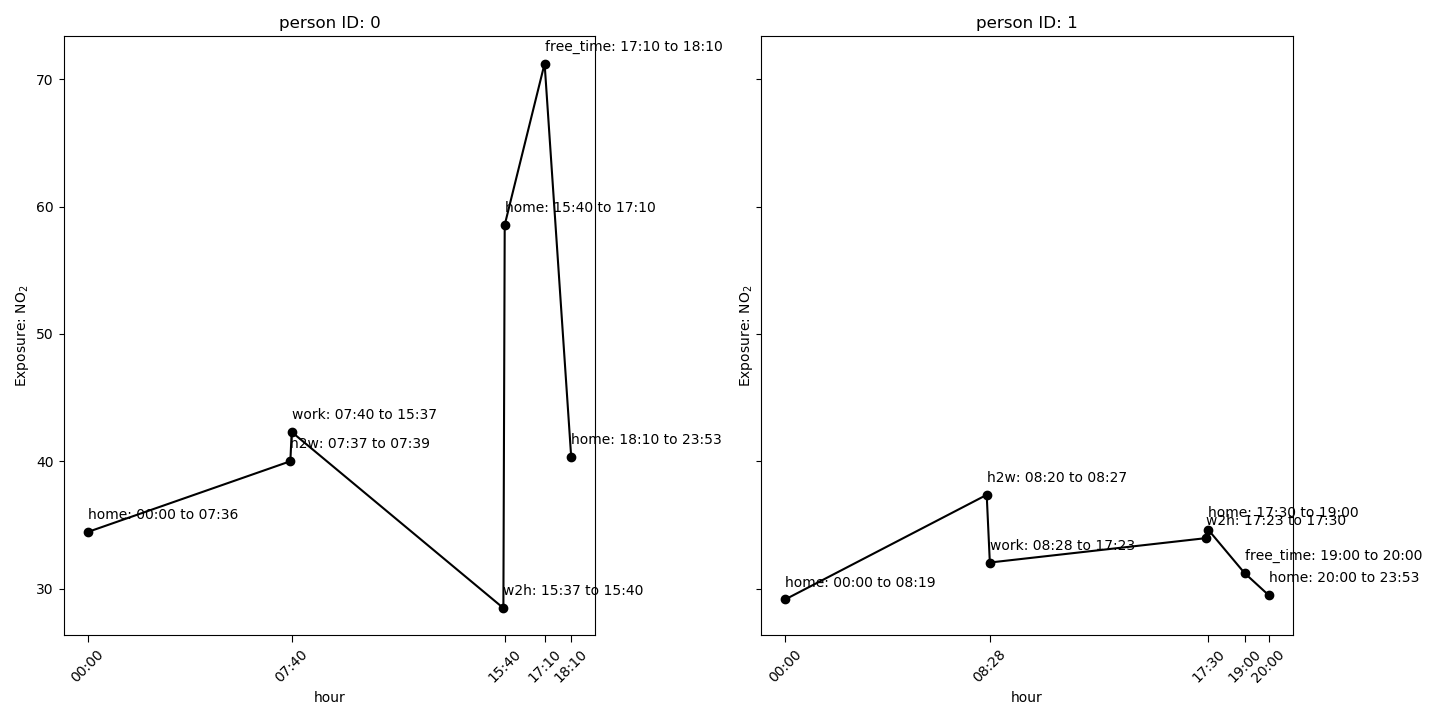
\includegraphics[width=12cm]{figure/exposure_act1.png}
    \caption{Example of assessed average exposure during each activity, in a single simulation instance. NO$_2$ exposure in $\mu g/m^3$ }
    \label{exp_act}
\end{figure}

\subsubsection{NO$_2$ prediction model}
We used the lightGBM (light gradient boosting machine) \citep{ke2017lightgbm} to predict hourly air quality from ground station measurements of Germany and Netherlands and geospatial predictors. LightGBM is a tree-based gradient boosting framework, which uses histogram-based algorithms to bin the continuous values of each feature \citep{ke2017lightgbm}. We compared the performance of LightGBM with XGBoost \citep{chen2015xgboost} with optimised hyper-parameters, and found the LightGBM obtained a slightly higher prediction accuracy (about 5\% lower in RMSE).

The predictors we used are highways, primary roads, local roads and industry areas in 100, 300, 500, 1000, 3000, 5000 m buffers; nightlight in 495, 750, 1050 m buffers; Tropomi L3 product (10km); elevation (30m); monthly wind speed and temperature of 2017 from the ERA-5Land simulation model. [details will be added].


\subsubsection{Exposure assessment model}
The exposure is assessed for each individual and scans over each activity in the activity schedule. The pseudo-code \cref{pc_e} shows the process. 
 
\begin{algorithm}[H]
 \KwData{temporal NO$_2$ maps, for each agent activity schedules and spatial locations associated with each activity in the schedule.}
 \KwResult{exposure assessed for each activity and for each person.}
 
 \For{each agent}{
 initialization\;
 exposure\_activity = 0 
 
 \For{each activity}{ 
    exposure\_activity $+=$ NO$_2$\_of\_corresponding\_time\_over spatial\_locations\_of\_the\_agent $\times$ activity\_duration
 }
exposure\_agent = exposure\_activity /time\_of\_all\_activities   
 }
 \caption{Exposure calculation, exposure\_agent indicates exposure calculated for each agent, exposure\_activity indicates exposure calculated for each activity in the schedule for each agent.}
 \label{pc_e}
\end{algorithm}


\subsection{Result}
\label{sec:result}

\subsubsection{Annually aggregated hourly prediction of NO$_2$}

\Cref{con} shows hourly NO$_2$ predicted using Light GBM. The error matrix is shown in table X.  

\begin{figure}[h]
    \centering
        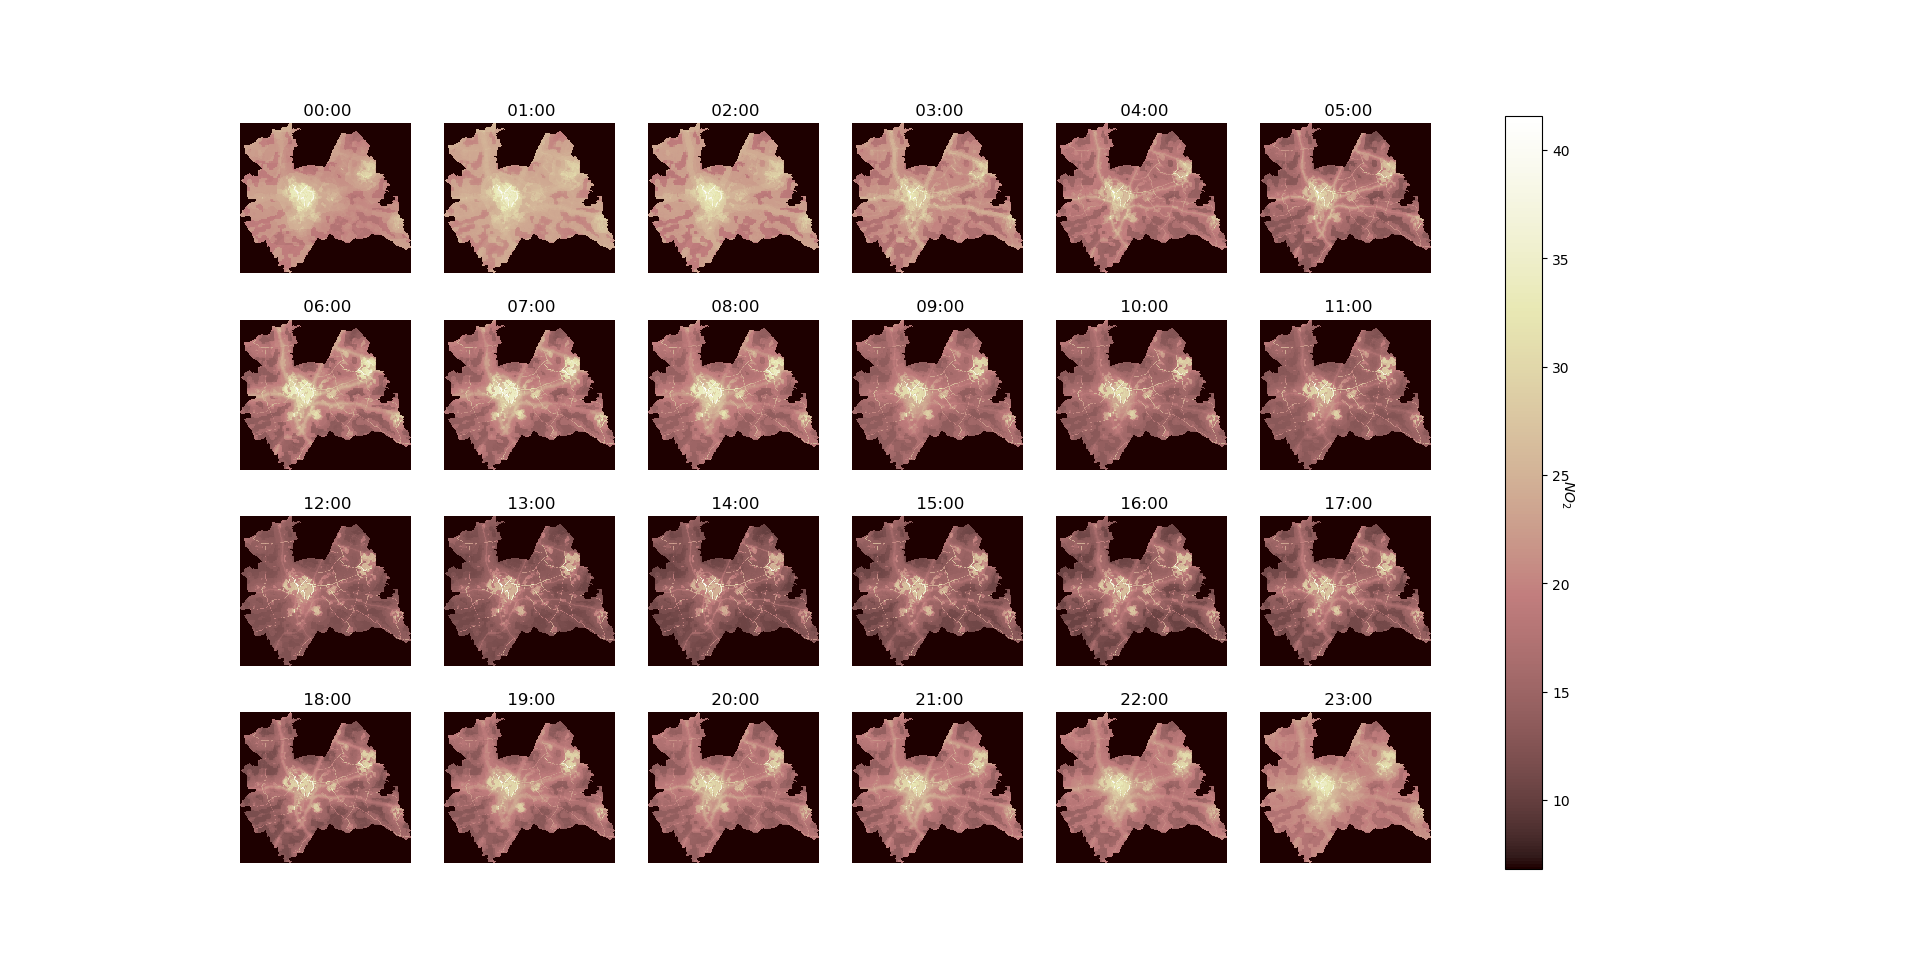
\includegraphics[scale = 0.3]{figure/prediUt.png}
    \caption{annually aggregated hourly NO$_2$ ($\mu g / m^3$) predicted for Utrecht.}
    \label{con}
\end{figure}

\subsubsection{Exposure calculated}

A example of exposure assessed using the model, for one of the activities: home to university \cref{sims}. The exposure assessed using true location is shown for comparison. It can be observed that the exposure calculated using the proposed model is close to the exposure calculated using the true location. Multiple simulations provide us an uncertainty measure.  
\begin{figure}[h]
    \centering
    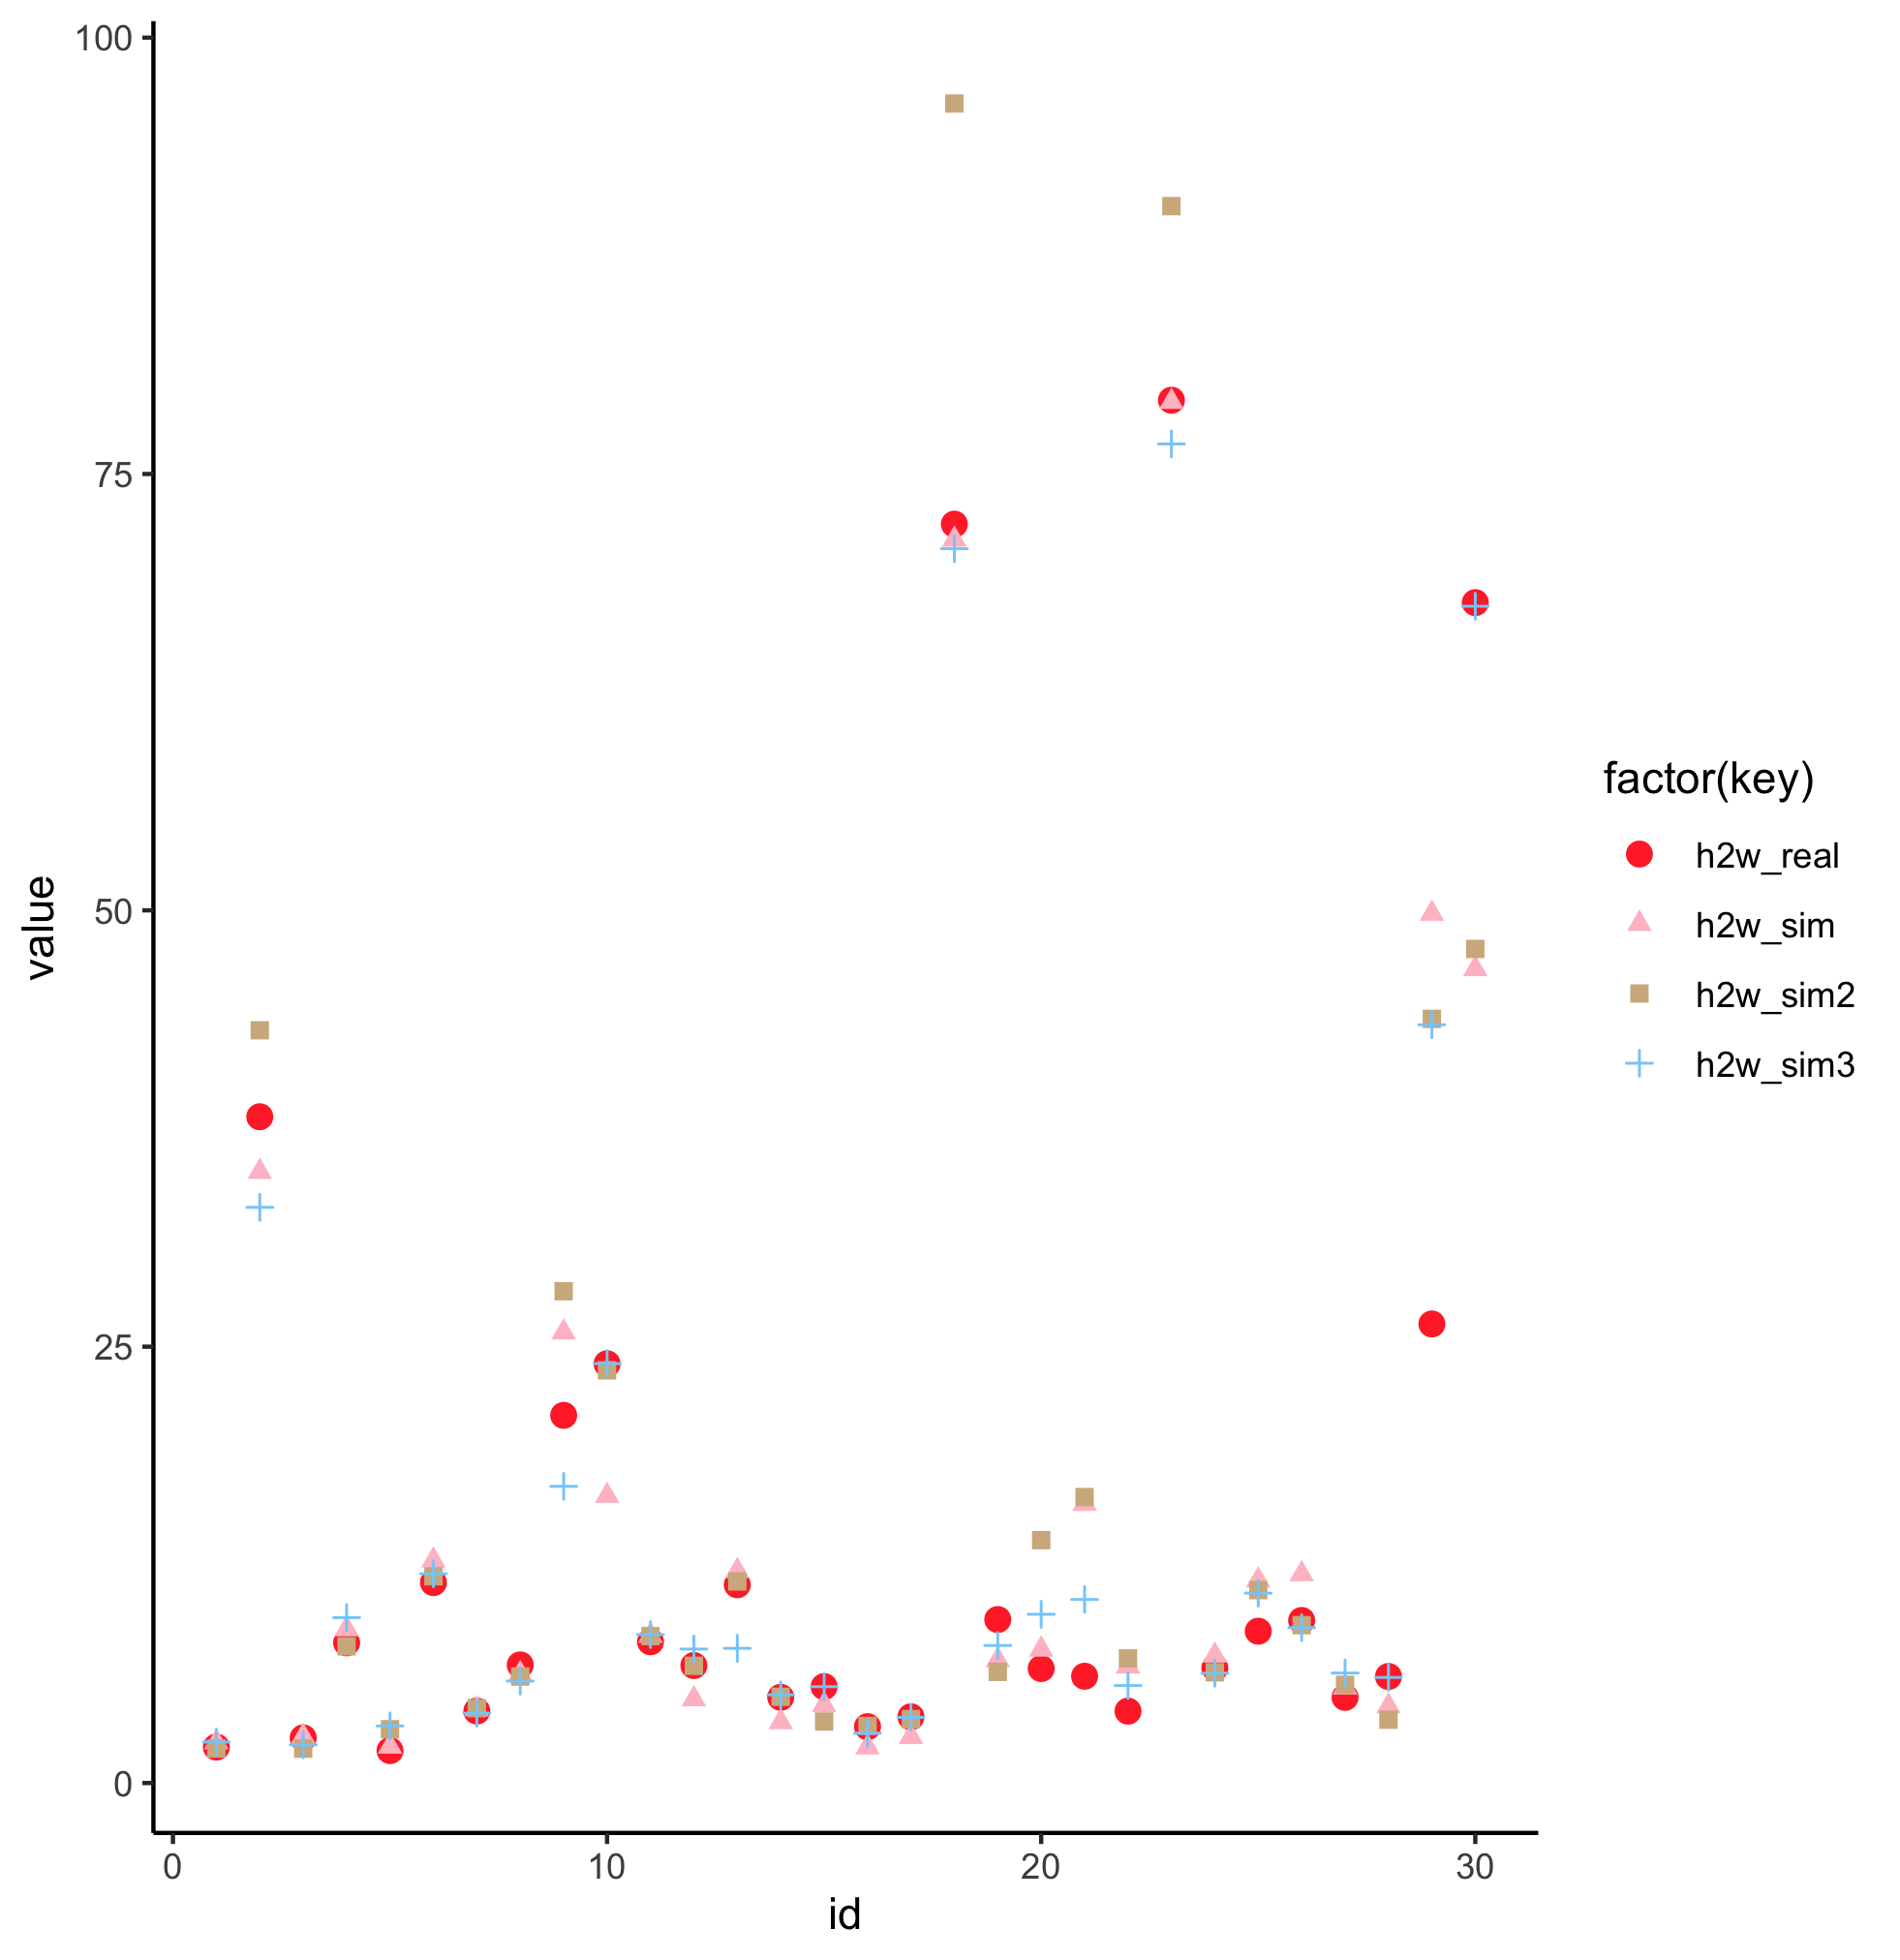
\includegraphics[width=8cm]{figure/sims.png}
    \caption{Exposure assessed for university, over the route home to university. The exposure is calculated as aggregating the NO$_2$ concentration along the route over the corresponding time span. The red dots indicate exposure assessed using real location, and others 3 times of simulated university locations and travel means.}
    \label{sims}
\end{figure}


\Cref{expmap} shows the exposure assessed for 49 students from the sub-population group "university students", where we know their home and collage/university locations. It can be observed that high exposures do not necessarily occur for people with high concentrations on home locations.
\begin{figure}[h]
    \centering
    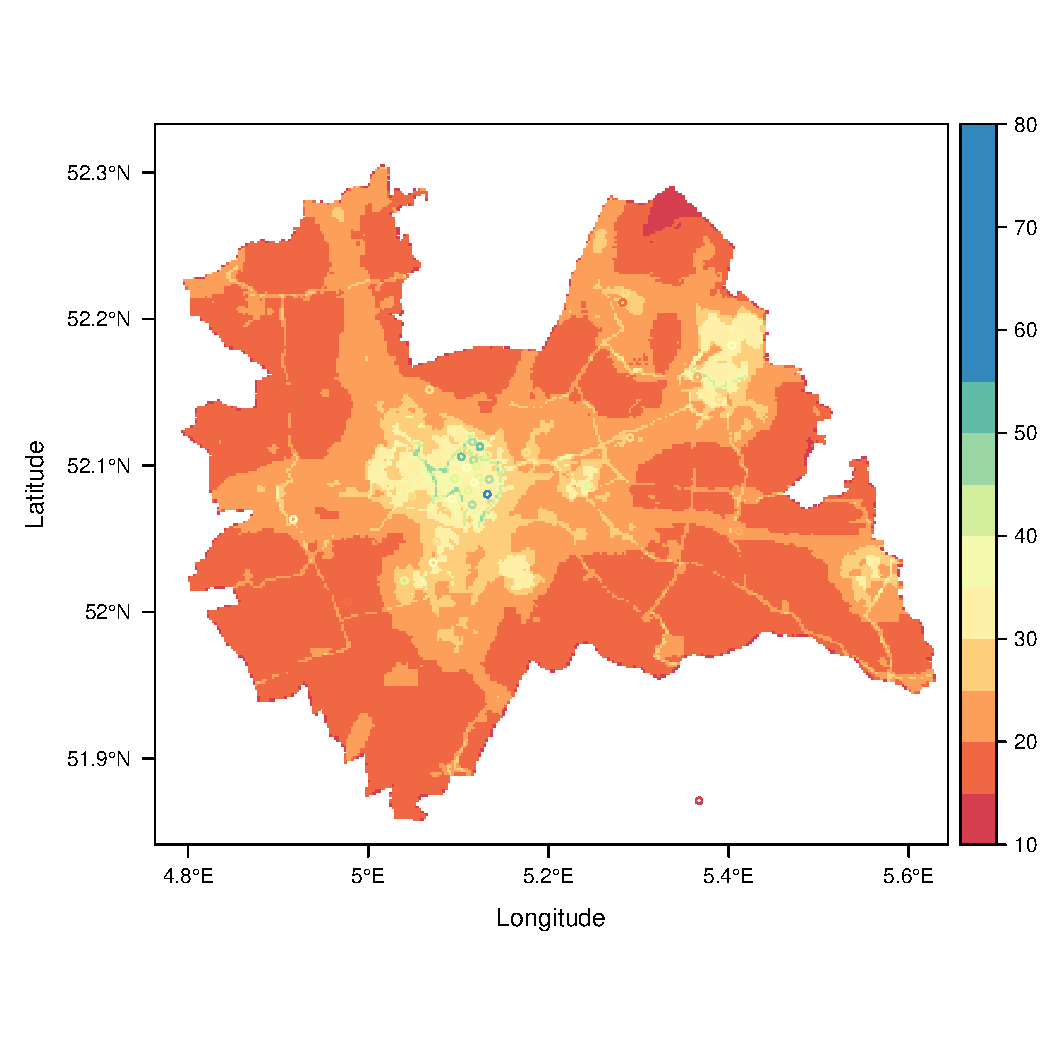
\includegraphics[width=8cm]{figure/utschoolmean2.pdf}
    \caption{Exposure assessed for the population group "University students", using the mean of all the iterations.  Background: annual mean NO$_2$ predictions for 2017, calculated by taking the average of all the annual hourly NO2 predictions.}
    \label{expmap}
\end{figure}



\section{Discussion}
\label{sec:dis}

\begin{figure}[!h]
    \centering
    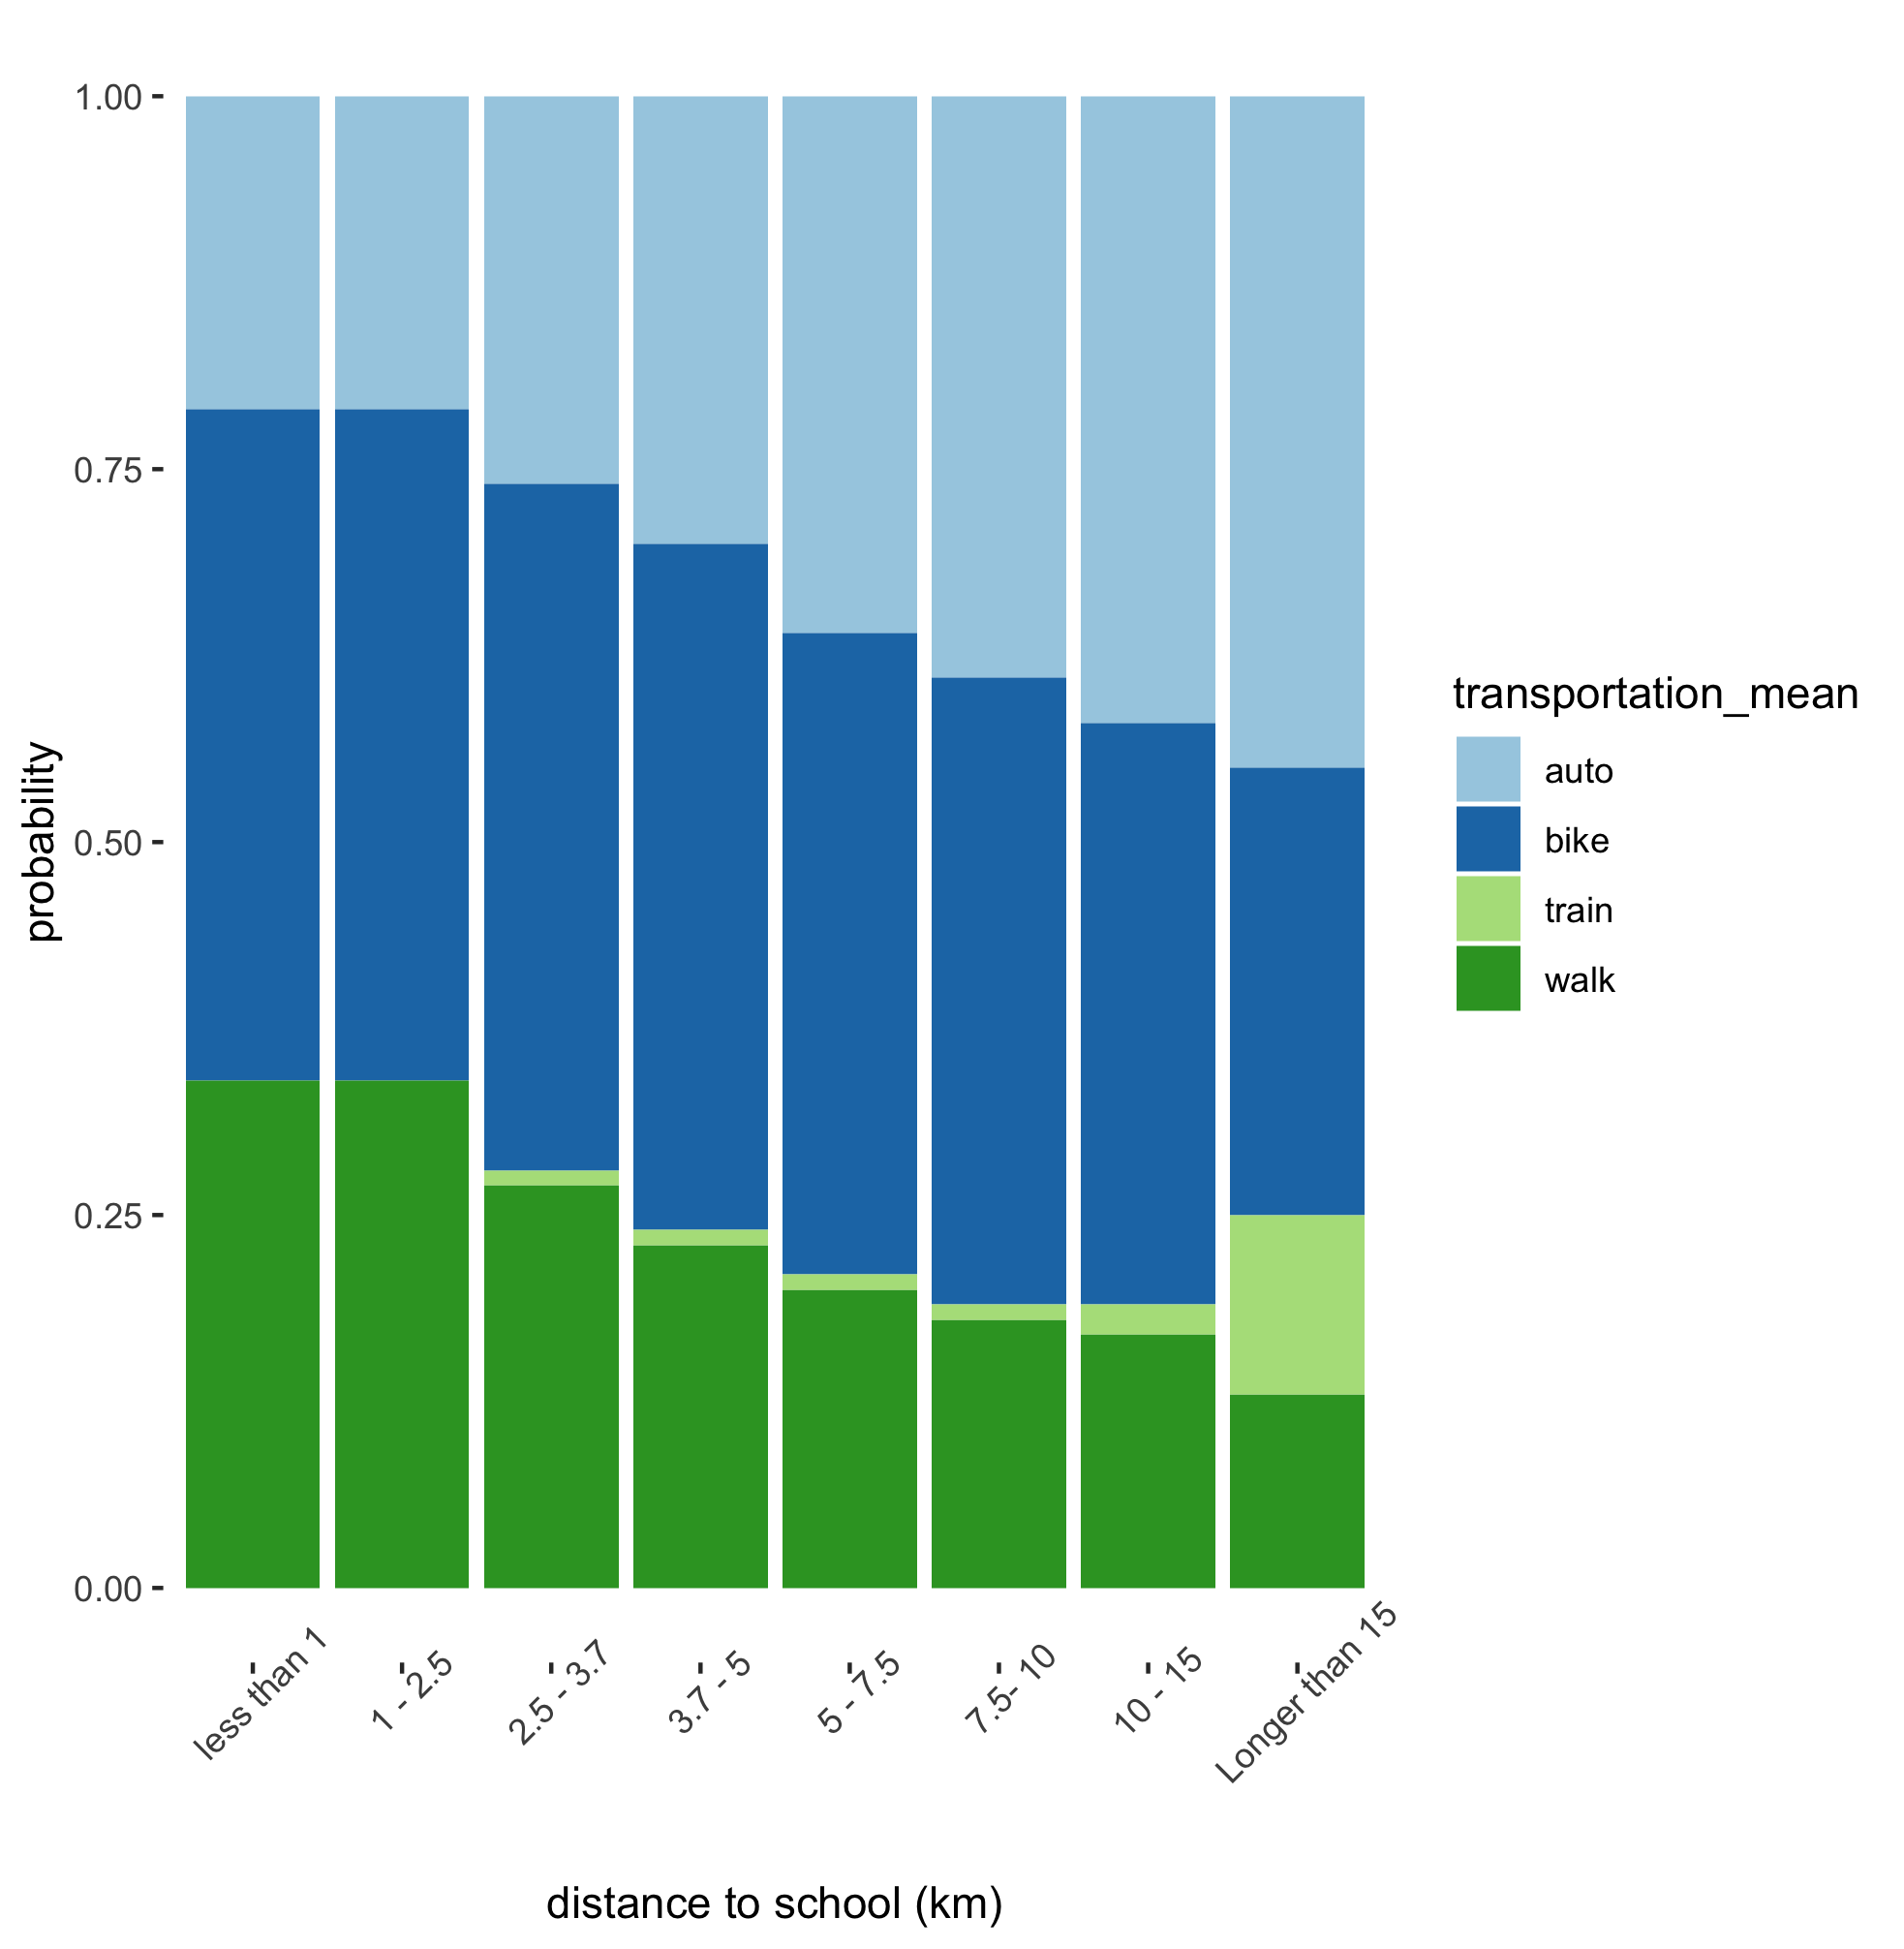
\includegraphics[width=8cm]{figure/ditance_vs_transmean_Uni.png}
    \caption{Probability of the transportation mean with regard to trip distance ranges for University students (older than 17). The trip distance ranges are re-scaled from the original travel distance. The transportation means are re-grouped from the transportation means in the Ovin survey.}
    \label{Uni_mode_dist}
\end{figure}

A major improvement of this work compared to recent activity-based exposure assessment models \citep{lu2019activity} is that it proposes the location and schedule simulation algorithms being explicitly basing on the probability distributions of the travel mean and maximum travel range of different population groups. Also, the departure times, free time activities, and the time for starting the free-time activities can all be sampled from a specific probability distribution. These greatly reduce the uncertainty in the activity simulation in general and for different population groups, which make it more suitable to be used in health studies and risk assessment. Compared to the proposed model, the framework of \citep{lu2019activity} consists of a complete random destination sampling procedure, a static activity schedule, and assumes one travel mode for all the individuals. 


The exposure calculation model iterate over each person and then aggregate the air pollution concentrations over the route of each activity of the person (with the indoor-outdoor ratio accounted). It is suitable for a relatively small population calculation. For a population larger than the number of time steps, an approach that iterate over each time step might be more efficient.  
%The model simulation for routes and schedules is fast, the only costly function is the nearest point searching. %

Our model relies on the distribution of the variables of travel behaviours and is therefore flexible and scalable as long as the data supports. It is flexible as it can potentially include any variable which influence the travel behaviour. For example, the probability of selecting a travel mean could be estimated using the relationships with other variables such as if the area is rural or urban, or the weather conditions, additional to what has been shown in our study case (based on e.g. age or if a person is a student or worker). The model is scalable means the model can be applied to any areas as long as the mobility information at the microcensus data level is available for the area. By design, the model focuses on land travel behaviour, i.e. we don't consider taking flight or long-distance ferries. The current model consider travel by train the same as travel by autovechicles (e.g. car, bus), in future we aim at a more sophisticated design for the train profile. 
 % Note: How is the train route calculated? If an agent (person) takes
  %a train, it is assumed he/she will firstly walk or cycle to the
  %nearest train station, and get off at the train station closest to the
  %destination location. (\emph{to be considered}). I intend to firstly
  %model within the Utrecht city, so all the destinations should be
  %constrained to a certain distance, therefore the mode: train has a
  %very small probability. This model may also be remove, then in
  %implementation i can simply replace train with autovehicles  .
    
\section{Conclusion}
\label{sec:con}

The method can potentially be applied to long-term, large-scale air pollution exposure assessment and for many other exposure assessment tasks, for example Ozone and Particulate Matters. The flexible input makes it convenient to assimilate diverse data collections.


\newpage
\bibliographystyle{plainnat}
\bibliography{ref}


\end{document}

\begin{table}[!htbp] \centering 
  \caption{Example activity schedule 1, h2w means "home to work", and w2h means "work to home". The "bicycle" indicates the transportation mean, which is generated from the activity model. The integer part indicates hours, and the digits indicate minutes in percentage, e.g., 9.89 is at around 9:54 am. (54 = 89*0.6). } 
  \label{schedule} 
\begin{tabular}{@{\extracolsep{5pt}} cccc} 
\\[-1.8ex]\hline 
\hline \\[-1.8ex] 
 & start\_time & end\_time & activity \\ 
\hline \\[-1.8ex] 
1 & $0$ & $9.89$ & home \\ 
2 & $9.90$ & $10.19$ & h2w\_bicycle \\ 
3 & $10.20$ & $17.10$ & work \\ 
4 & $17.11$ & $17.39$ & w2h\_bicycle \\ 
5 & $17.40$ & $18.89$ & home \\ 
6 & $18.90$ & $19.89$ & sports \\ 
7 & $19.90$ & $23.90$ & home \\ 
\hline \\[-1.8ex] 
\end{tabular} 
\end{table}

\begin{table}[!htbp] \centering 
  \caption{Example activity schedule 2, for notations please refer to \cref{schedule}. "Auto" indicates all the other vehicles, of course, for U17, they are not driving themselves.} 
  \label{schedule2} 
\begin{tabular}{@{\extracolsep{5pt}} cccc} 
\\[-1.8ex]\hline 
\hline \\[-1.8ex] 
 & start\_time & end\_time & activity \\ 
\hline \\[-1.8ex] 
1 & $0$ & $9.33$ & home \\ 
2 & $9.34$ & $9.60$ & h2w\_auto \\ 
3 & $9.61$ & $16.43$ & work \\ 
4 & $16.44$ & $16.69$ & w2h\_auto \\ 
5 & $16.70$ & $18.19$ & home \\ 
6 & $18.20$ & $19.19$ & sports \\ 
7 & $19.20$ & $23.90$ & home \\ 
\hline \\[-1.8ex] 
\end{tabular} 
\end{table} 


\subsection{Implementation}
\begin{enumerate}
\def\labelenumi{\arabic{enumi}.}
\item
  Activities:
  \emph{Work-day activities:} 1) home, 2) home to work, 3) work, 4) work
  to home, 5) sports. The assumption for sports is that it occurs in the
  morning or evening, and it occurs either 1 hour before departure to
  work or 1 hour after come back home from work.

  \emph{Weekend activity}: 1) shopping, 2) random walk 
\item
  A \textbf{probailistic} model: the components below are probabilistic,
  and the distributions can come for activity surveys or literature.

  1) \underline{Time schedule:} please see section 2 for the activities.
  The departure times to work and back from home are probabilisitic. By
  default, a gaussian distribution is used (e..g with mean 8 and
  standard deviation 0.5 for going to work). In our implementation, the
  distributions of departure times are fitted (characterised) from human
  activity surveys (please see section 4 below). The distributions are
  fitted for each population group.

  2) \underline{Unknown destination locations:} For large-population
  activity modeling, it is commonly the case that the specific
  destination location (e.g. work location, sport centres) are unknown
  for each individual. However, the information for the entire locations
  (e.g. sport centres, work buildings, universities, schools) are
  becoming more comprehensive. In many countries, this part of
  information can be acquired from OpenStreetMaps. In this study, we
  select potential locations by proabilisticly sampling the maximum trip
  distance and only randomly select locations within the Euclidean
  distance of the maximum trip distance. If there is no destination
  points within the sampled maximum trip distance, the nearest
  destination point is used. The number of total selected destination
  points serve as an uncertainty indicator in the situation of unknown
  destination locations, in each simulation run.

  3) \emph{\underline{Means of commuting}} (currently: (train),
  autovehicles (car, bus, tram), bike, on foot): are deteremined based
  on travel distance. Based on the population group (e.g. school
  student) and the travel purpose (to school), the probability that a
  certain travel mean is taken is calculated (e.g. 0.3 for on foot and
  0.6 for biking, 0.1 for taking a bus or car and 0 for others),
  according to which a travel mode is sampled in each simulation. The
  commuting routes are queried from OpenStreetMaps.

  Note: {[}How is the train route calculated? If an agent (person) takes
  a train, it is assumed he/she will firstly walk or cycle to the
  nearest train station, and get off at the train station closest to the
  destination location. (\emph{to be considered}). I intend to firstly
  model within the Utrecht city, so all the destinations should be
  constrained to a certain distance, therefore the mode: train has a
  very small probability. This model may also be remove, then in
  implementation i can simply replace train with autovehicles{]} .
\item
  Implementation:

  Population group implemented are: school student (U17) , University
  student (students older than 18 years old, Uni), part-time worker
  (PW), full-time worker (FW).

  There is a conceptural default implemented in our model which is
  described in table 1. In our case-study (Utrecht) implementation, they
  are characterised from Dutch national activity surveys (OVin). The
  process is: 1) we select a profile (e.g. Univeristy student) and a
  purpose (e.g. go to work), 2) we fit the distribution of the selected
  data. 3) At each simulation, we sample one value from the
  distribution. Specifications are described below:

  \textbf{Destination location selection:}
\end{enumerate}
